% !TEX root = ../main.tex

\section{Method of Disks/Washers (Perpendicular to the $x$-axis)}

\begin{myframe}[arc=10pt,auto outer arc]
		\centering
		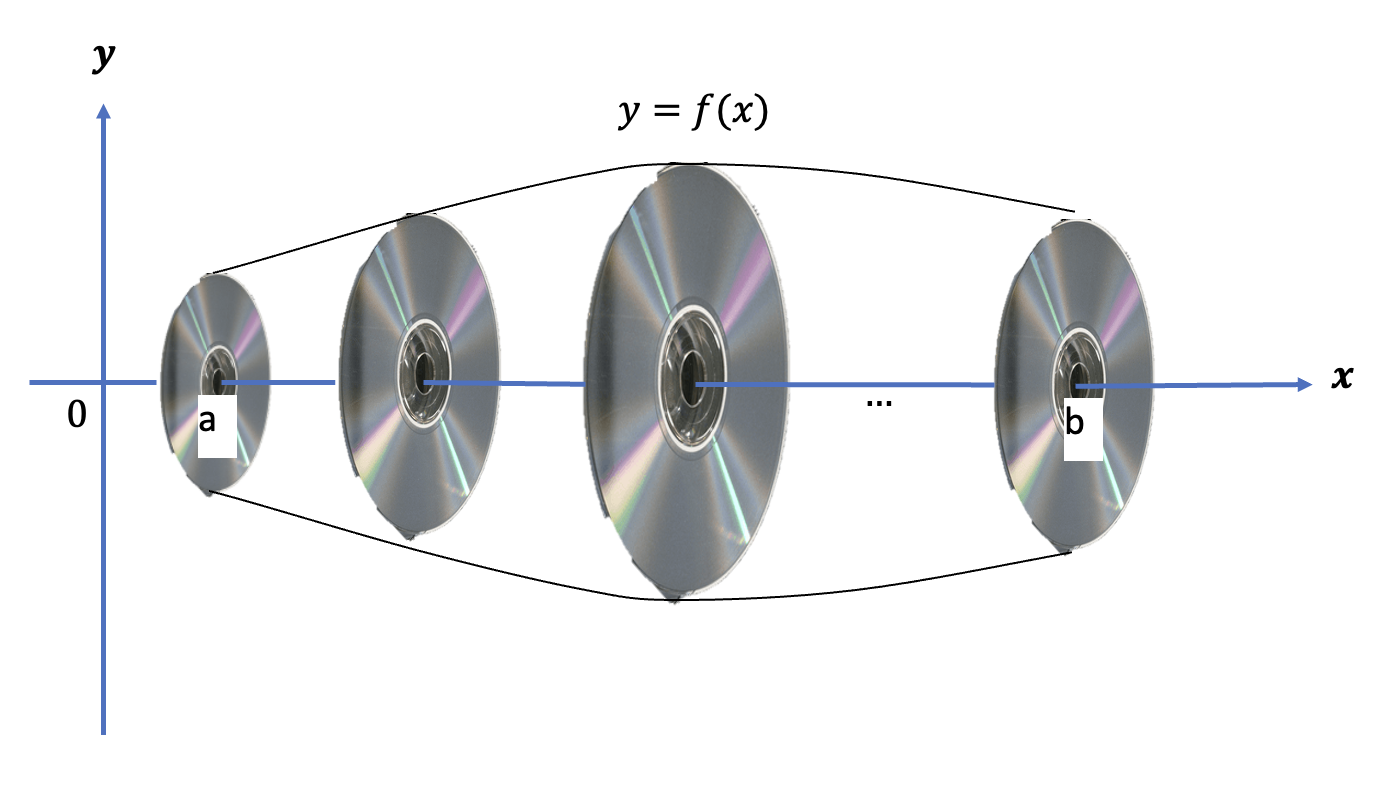
\includegraphics[width=0.7\linewidth]{chapter5/disc}
		
		\begin{enumerate}
			\item $\displaystyle \textrm{Area} = \pi\left(f(x) - 0\right)^2 = \pi\left(f(x) \right)^2$
			\item $\displaystyle \textrm{Volume} = \pi \int_{x=a}^b \left[ f(x) \right]^2 \, dx$
		\end{enumerate}
	
\end{myframe}

\problemans%
{Find the volume of the solid that is obtained when the region \\
	under the curve $y=\sqrt{x}$ over the interval $[1, 4]$  \\
	is revolved about the $x$-axis. 
}%
{$\displaystyle \frac{15}{2} \pi$}%

\newpage
\problemans%
{Find the volume of the solid that is obtained when the region \\
between the graph $\displaystyle f(x)=\frac{1}{2} + x^2$ and $g(x)=x$ over the interval $[0, 2]$ \\
is revolved about the $x$-axis.}%
{$\displaystyle \frac{69}{10}\pi$}%

\newpage
\problemans%
{Find the volume of the solid that is obtained when the region \\
	bounded by the graph $x=y^2$ and $y=x^2$ \\
	is revolved about the $x$-axis.
}%
{$\displaystyle \frac{3}{10} \pi$}%

\newpage
\problemans%
{Find the volume of the solid that is obtained when the region \\
	bounded by the graph $y=x^2$ and $y=x^3$ \\
	is revolved about the line $y=-1$. 
}%
{$\displaystyle \frac{47}{210}\pi$}%

%%%% GUIDES
\qrfigure{chapter5/qr/Method-of-Disks-Washers-Perpendicular-to-the-x-axis}{Scan for guides}

%-------------------------------------------------------
\makenewpage
\section{Method of Disks/Washers (Perpendicular to the $y$-axis)}

\begin{myframe}[arc=10pt,auto outer arc]
	\centering
	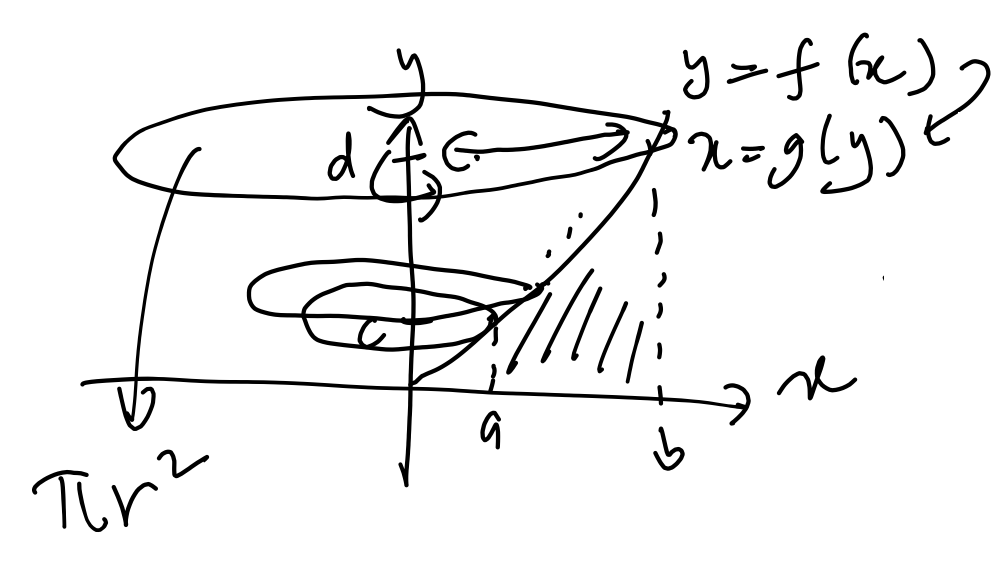
\includegraphics[width=0.7\linewidth]{chapter5/discy}
	
	\begin{enumerate}
		\item $\displaystyle \textrm{Area} = \pi\left(g(y) - 0\right)^2 = \pi \left[g(y)\right]^2$
		\item $\displaystyle \textrm{Volume} = \pi \int_{y=c}^d \left[ g(y) \right]^2 \, dy$
	\end{enumerate}
	
\end{myframe}

\problemans%
{Find the volume of the solid that is generated when the region \\
	enclosed by $y=\sqrt{x}$, $y=2$ and $x=0$ \\
	is revolved about the $y$-axis. 
}%
{$\displaystyle \frac{32}{5}\pi$}%

\newpage
\problemans%
{Find the volume of the solid that is generated when the region \\
	enclosed by $x=y^2$ and $y=x^2$ \\
	is revolved about the $y$-axis.   
}%
{$\displaystyle \frac{3}{10}\pi$}%

\newpage
\problemans%
{Find the volume of the solid that is generated when the region \\ 
	bounded by $y=x^2$ and $y=x^3$\\
	is revolved about the line $x=-1$.  
}%
{$\displaystyle \frac{4}{15}\pi$}%

%%%% GUIDES
\qrfigure{chapter5/qr/Method-of-Disks-Washers-Perpendicular-to-the-y-axis}{Scan for guides}





